%%%%%%%%%%%%%%%%%%%%%%%%%%%%%%%%%%%%%%%%%%%%%%%%%%%%%%%%%%%%%%%%%%%%%
%% This is a (brief) model paper using the achemso class
%% The document class accepts keyval options, which should include
%% the target journal and optionally the manuscript type. 
%%%%%%%%%%%%%%%%%%%%%%%%%%%%%%%%%%%%%%%%%%%%%%%%%%%%%%%%%%%%%%%%%%%%%
\documentclass[journal=jceda8,manuscript=article]{achemso}

%%%%%%%%%%%%%%%%%%%%%%%%%%%%%%%%%%%%%%%%%%%%%%%%%%%%%%%%%%%%%%%%%%%%%
%% Place any additional packages needed here.  Only include packages
%% which are essential, to avoid problems later. Do NOT use any
%% packages which require e-TeX (for example etoolbox): the e-TeX
%% extensions are not currently available on the ACS conversion
%% servers.
%%%%%%%%%%%%%%%%%%%%%%%%%%%%%%%%%%%%%%%%%%%%%%%%%%%%%%%%%%%%%%%%%%%%%
\usepackage[version=3]{mhchem} % Formula subscripts using \ce{}
\usepackage{hyperref}
%%%%%%%%%%%%%%%%%%%%%%%%%%%%%%%%%%%%%%%%%%%%%%%%%%%%%%%%%%%%%%%%%%%%%
%% If issues arise when submitting your manuscript, you may want to
%% un-comment the next line.  This provides information on the
%% version of every file you have used.
%%%%%%%%%%%%%%%%%%%%%%%%%%%%%%%%%%%%%%%%%%%%%%%%%%%%%%%%%%%%%%%%%%%%%
%%\listfiles

%%%%%%%%%%%%%%%%%%%%%%%%%%%%%%%%%%%%%%%%%%%%%%%%%%%%%%%%%%%%%%%%%%%%%
%% Place any additional macros here.  Please use \newcommand* where
%% possible, and avoid layout-changing macros (which are not used
%% when typesetting).
%%%%%%%%%%%%%%%%%%%%%%%%%%%%%%%%%%%%%%%%%%%%%%%%%%%%%%%%%%%%%%%%%%%%%
\newcommand*\mycommand[1]{\texttt{\emph{#1}}}

%%%%%%%%%%%%%%%%%%%%%%%%%%%%%%%%%%%%%%%%%%%%%%%%%%%%%%%%%%%%%%%%%%%%%
%% Meta-data block
%% ---------------
%% Each author should be given as a separate \author command.
%%
%% Corresponding authors should have an e-mail given after the author
%% name as an \email command. Phone and fax numbers can be given
%% using \phone and \fax, respectively; this information is optional.
%%
%% The affiliation of authors is given after the authors; each
%% \affiliation command applies to all preceding authors not already
%% assigned an affiliation.
%%
%% The affiliation takes an option argument for the short name.  This
%% will typically be something like "University of Somewhere".
%%
%% The \altaffiliation macro should be used for new address, etc.
%% On the other hand, \alsoaffiliation is used on a per author basis
%% when authors are associated with multiple institutions.
%%%%%%%%%%%%%%%%%%%%%%%%%%%%%%%%%%%%%%%%%%%%%%%%%%%%%%%%%%%%%%%%%%%%%
%\author{Peng Liu}
%\affiliation[Pitt]{Department of Chemistry, University of Pittsburgh}
\author{David Ryan Koes}
\email{dkoes@pitt.edu}
\affiliation[Pitt]{Department of Computational and Systems Biology, University of Pittsburgh}

%%%%%%%%%%%%%%%%%%%%%%%%%%%%%%%%%%%%%%%%%%%%%%%%%%%%%%%%%%%%%%%%%%%%%
%% The document title should be given as usual. Some journals require
%% a running title from the author: this should be supplied as an
%% optional argument to \title.
%%%%%%%%%%%%%%%%%%%%%%%%%%%%%%%%%%%%%%%%%%%%%%%%%%%%%%%%%%%%%%%%%%%%%
\title[3Dmol.js Learning Environment]
  {The 3Dmol.js learning environment: a classroom response system for 3D chemical structures}

%%%%%%%%%%%%%%%%%%%%%%%%%%%%%%%%%%%%%%%%%%%%%%%%%%%%%%%%%%%%%%%%%%%%%
%% Some journals require a list of abbreviations or keywords to be
%% supplied. These should be set up here, and will be printed after
%% the title and author information, if needed.
%%%%%%%%%%%%%%%%%%%%%%%%%%%%%%%%%%%%%%%%%%%%%%%%%%%%%%%%%%%%%%%%%%%%%
\keywords{audience response system, clickers, active learning}

%%%%%%%%%%%%%%%%%%%%%%%%%%%%%%%%%%%%%%%%%%%%%%%%%%%%%%%%%%%%%%%%%%%%%
%% The manuscript does not need to include \maketitle, which is
%% executed automatically.
%%%%%%%%%%%%%%%%%%%%%%%%%%%%%%%%%%%%%%%%%%%%%%%%%%%%%%%%%%%%%%%%%%%%%
\begin{document}

%%%%%%%%%%%%%%%%%%%%%%%%%%%%%%%%%%%%%%%%%%%%%%%%%%%%%%%%%%%%%%%%%%%%%
%% The "tocentry" environment can be used to create an entry for the
%% graphical table of contents. It is given here as some journals
%% require that it is printed as part of the abstract page. It will
%% be automatically moved as appropriate.
%%%%%%%%%%%%%%%%%%%%%%%%%%%%%%%%%%%%%%%%%%%%%%%%%%%%%%%%%%%%%%%%%%%%%
\begin{tocentry}
    \includegraphics[height=1.25in]{handheld}
\end{tocentry}

%%%%%%%%%%%%%%%%%%%%%%%%%%%%%%%%%%%%%%%%%%%%%%%%%%%%%%%%%%%%%%%%%%%%%
%% The abstract environment will automatically gobble the contents
%% if an abstract is not used by the target journal.
%%%%%%%%%%%%%%%%%%%%%%%%%%%%%%%%%%%%%%%%%%%%%%%%%%%%%%%%%%%%%%%%%%%%%
\begin{abstract}
Classroom response systems are an important tool in many active learning pedagogies.  They support real-time feedback on student learning and promote student engagement, even in large classrooms, by allowing instructors to solicit an answer to a question from all students and show the results. Existing classroom response systems are general purpose and not tailored to the specific needs of a chemistry classroom.  In particular, it is not easy to deploy molecular representations except as static images. Here we present the 3Dmol.js learning environment, a classroom response system that uses the open source web-based 3Dmol.js JavaScript framework to provide interactive viewing and querying of 3D molecules.  3Dmol.js is available under a BSD 3-clause open source license, and the learning environment features are all available through \url{http://3dmol.csb.pitt.edu/} without any software installation required.
\end{abstract}

%%%%%%%%%%%%%%%%%%%%%%%%%%%%%%%%%%%%%%%%%%%%%%%%%%%%%%%%%%%%%%%%%%%%%
%% Start the main part of the manuscript here.
%%%%%%%%%%%%%%%%%%%%%%%%%%%%%%%%%%%%%%%%%%%%%%%%%%%%%%%%%%%%%%%%%%%%%
\section{Introduction}
Active learning is ``the process of having students engage in some activity that forces them to reflect upon ideas and how they are using those ideas.''\cite{collins2011greenwood}  The application of active learning pedagogies results in significant improvements in learning outcomes in science classrooms\cite{michael2006s,deslauriers2011improved,armbruster2009active}, including organic chemistry classes\cite{jeske2019collaborative,decicco2019clickers,webbased}.  One popular active learning method is the use of classroom response systems\cite{martyn2007clickers}, also known as audience/student/personal response systems or ``clickers.''  In these systems, the instructor poses a question and students answer using a personal device, either a dedicate piece of hardware (a ``clicker'') or a web-enabled device such as a smartphone or laptop\cite{webbased}.  Students answer anonymously and the collated answers are shown to the class to enable further discussion.  In a meta-analysis\cite{hunsu2016meta} of 53 studies, the use of classroom response systems was found to produce a small, but statistically significant, benefit on cognitive outcomes and a larger benefit on non-cognitive outcomes, such as the students' enjoyment of the class and ranking of the instructor.

The use of classroom response systems in the chemistry classroom is growing, particular for large classes\cite{gibbons2017chasm,woelk2008optimizing}.  However, general-purpose software not designed specifically for chemistry is often used, reducing the efficacy of the system\cite{webbased}.  Importantly, we are not aware of any system that seamlessly integrates 3D chemical structures, which are important for engaging students and enabling spatial learning\cite{viz32class}.  To address this need, we have extended the 3Dmol.js\cite{rego20153dmol} JavaScript library for online molecular visualization to include a learning environment with classroom response system features.  We next describe how these features work and discuss future directions.

\begin{figure}
    \centering
    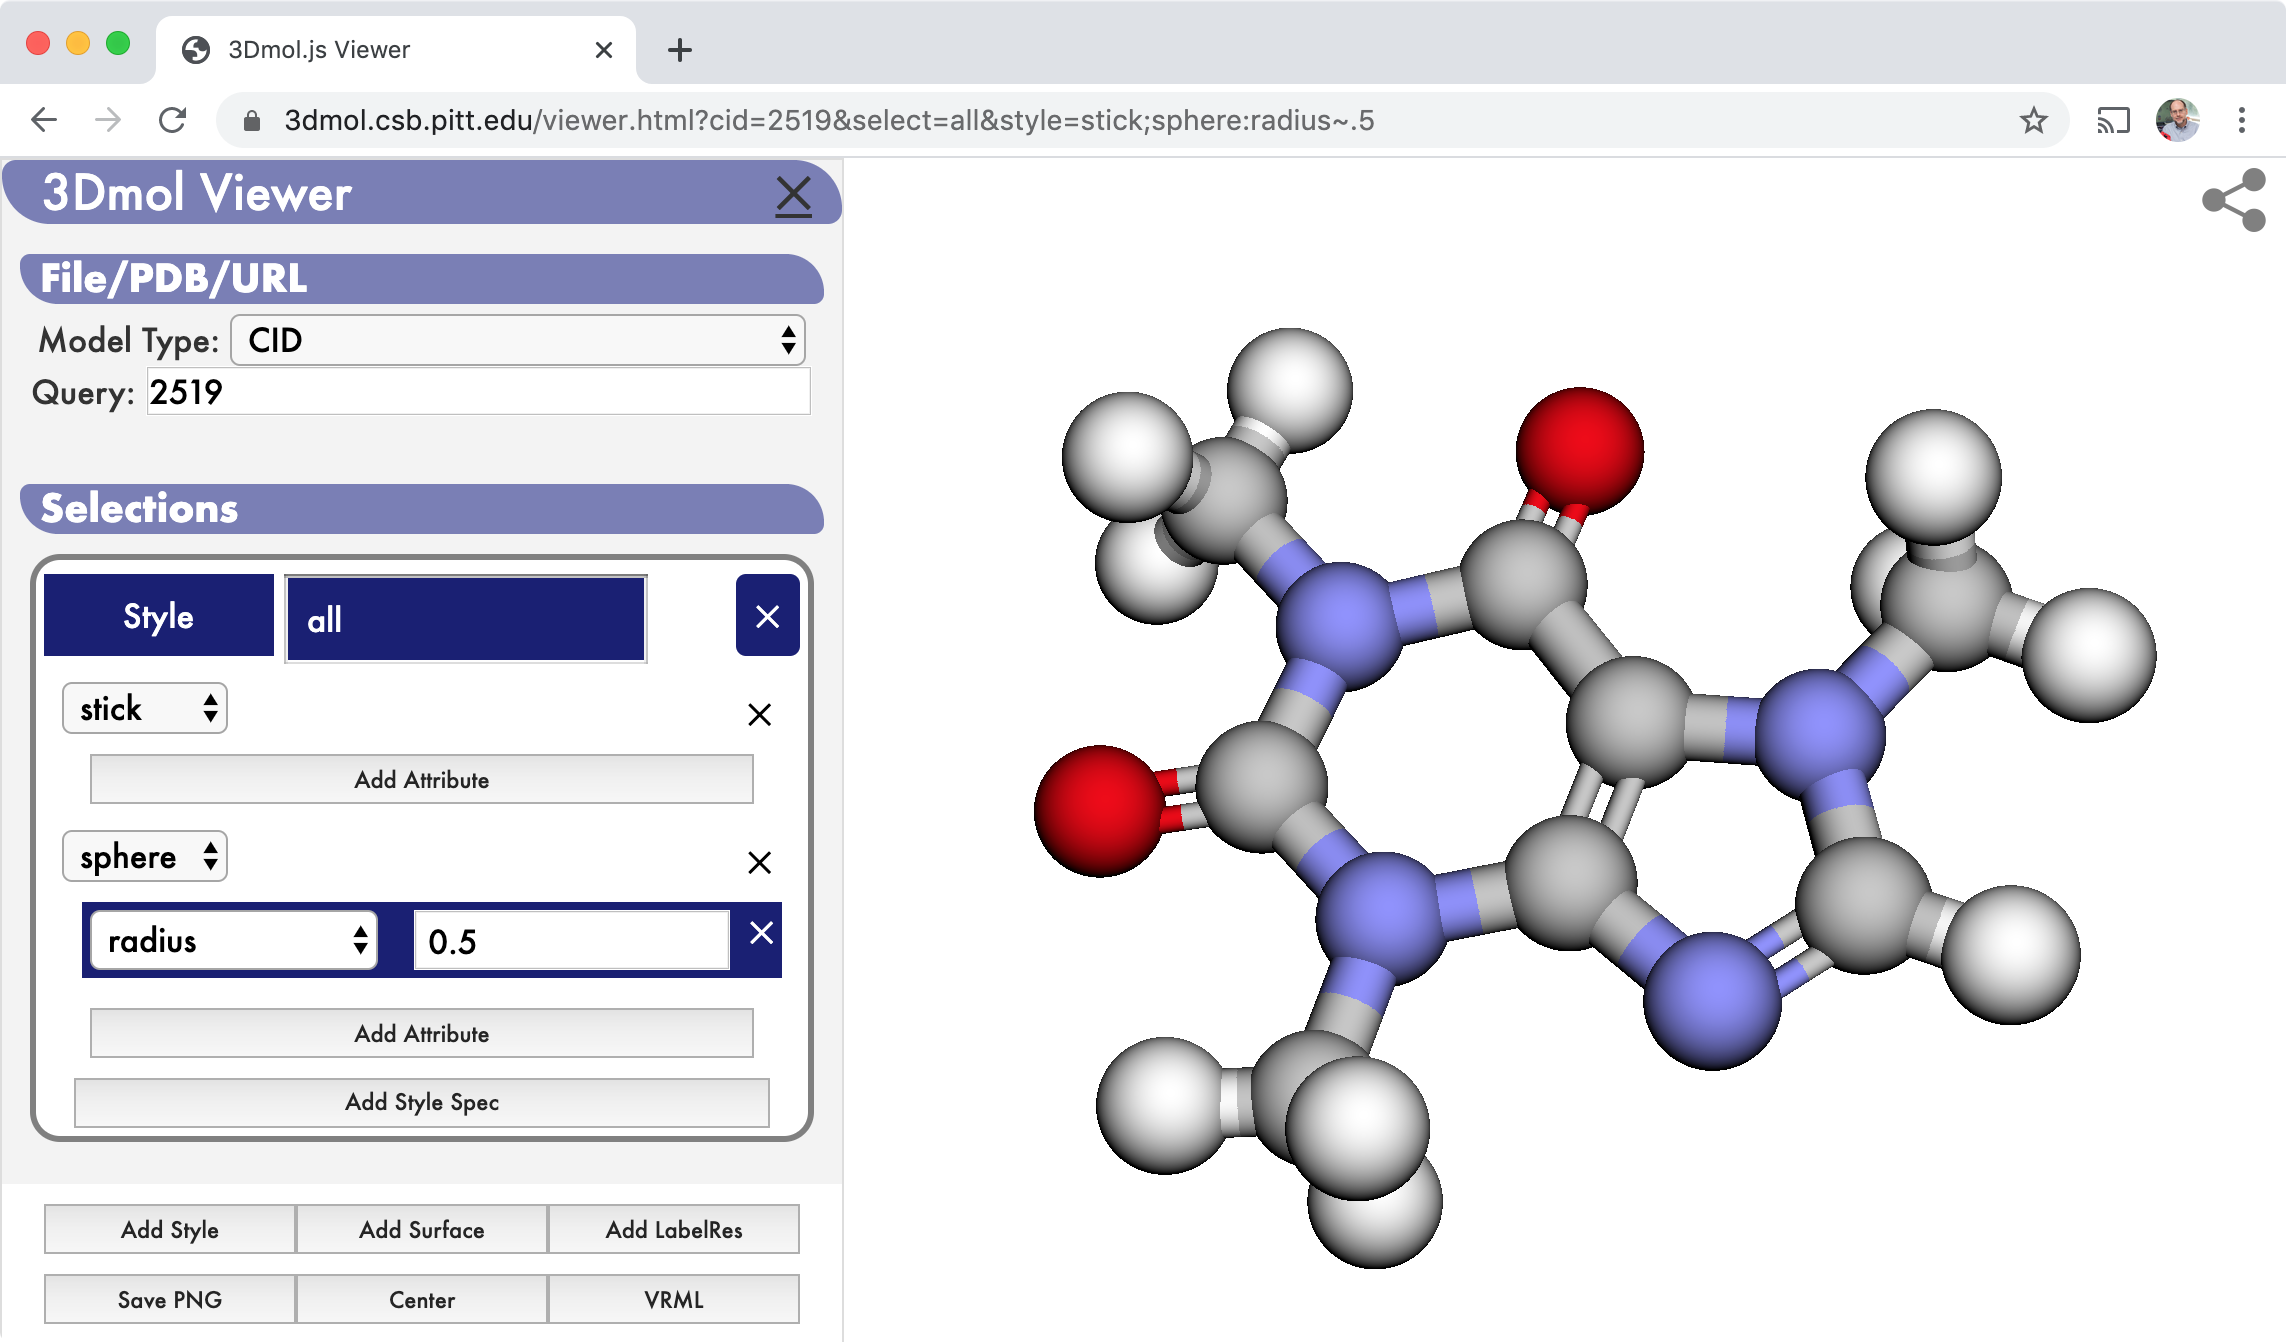
\includegraphics[width=\linewidth]{viewer}
    \caption{The 3Dmol.js viewer.  The edit panel (left) is shown and is used to load a molecule, in this case compound id 2519 from PubChem, and set the style.  The result can be accessed at the URL \url{https://3dmol.csb.pitt.edu/viewer.html?cid=2519&select=all&style=stick;sphere:radius~.5}}
    \label{fig:viewer}
\end{figure}

\section{3Dmol.js Learning Environment}

3Dmol.js\cite{rego20153dmol} is a WebGL-based JavaScript library for hardware-accelerated online molecular graphics.  It supports most molecular file formats and visualization styles, including support for volumetric data (e.g. cube files) and simulation data (e.g. AMBER\cite{case2005amber} or GROMACS\cite{van2005gromacs} data).  In addition to its full-featured JavaScript API, 3Dmol.js offers an embedding API, where a molecular view can be added to a web page by inserting a single \texttt{div} statement, and a URL-based hosted viewer API. The hosted viewer (\url{http://3dmol.csb.pitt.edu/viewer.html}) is specifically designed so that all information to display the current molecular view is included in the URL.  That is, having constructed a scene by loading the appropriate molecular data and applying the desired styles using the provided edit panel (Figure~\ref{fig:viewer}), it is possible to share the URL with students (e.g. as a QR code) so they can see the identical scene and interact with it.  Molecular data is loaded into the viewer by specifying a PubChem compound id (the PubChem entry must have an associated 3D structure), a Protein Data Bank identifier, or a URL to an externally hosted file.    We have added functionality to the 3Dmol.js API and hosted viewer to create a learning environment that can be used as a classroom response system where students answer queries by clicking on atoms of a 3D molecule.

\begin{figure}
    \centering
    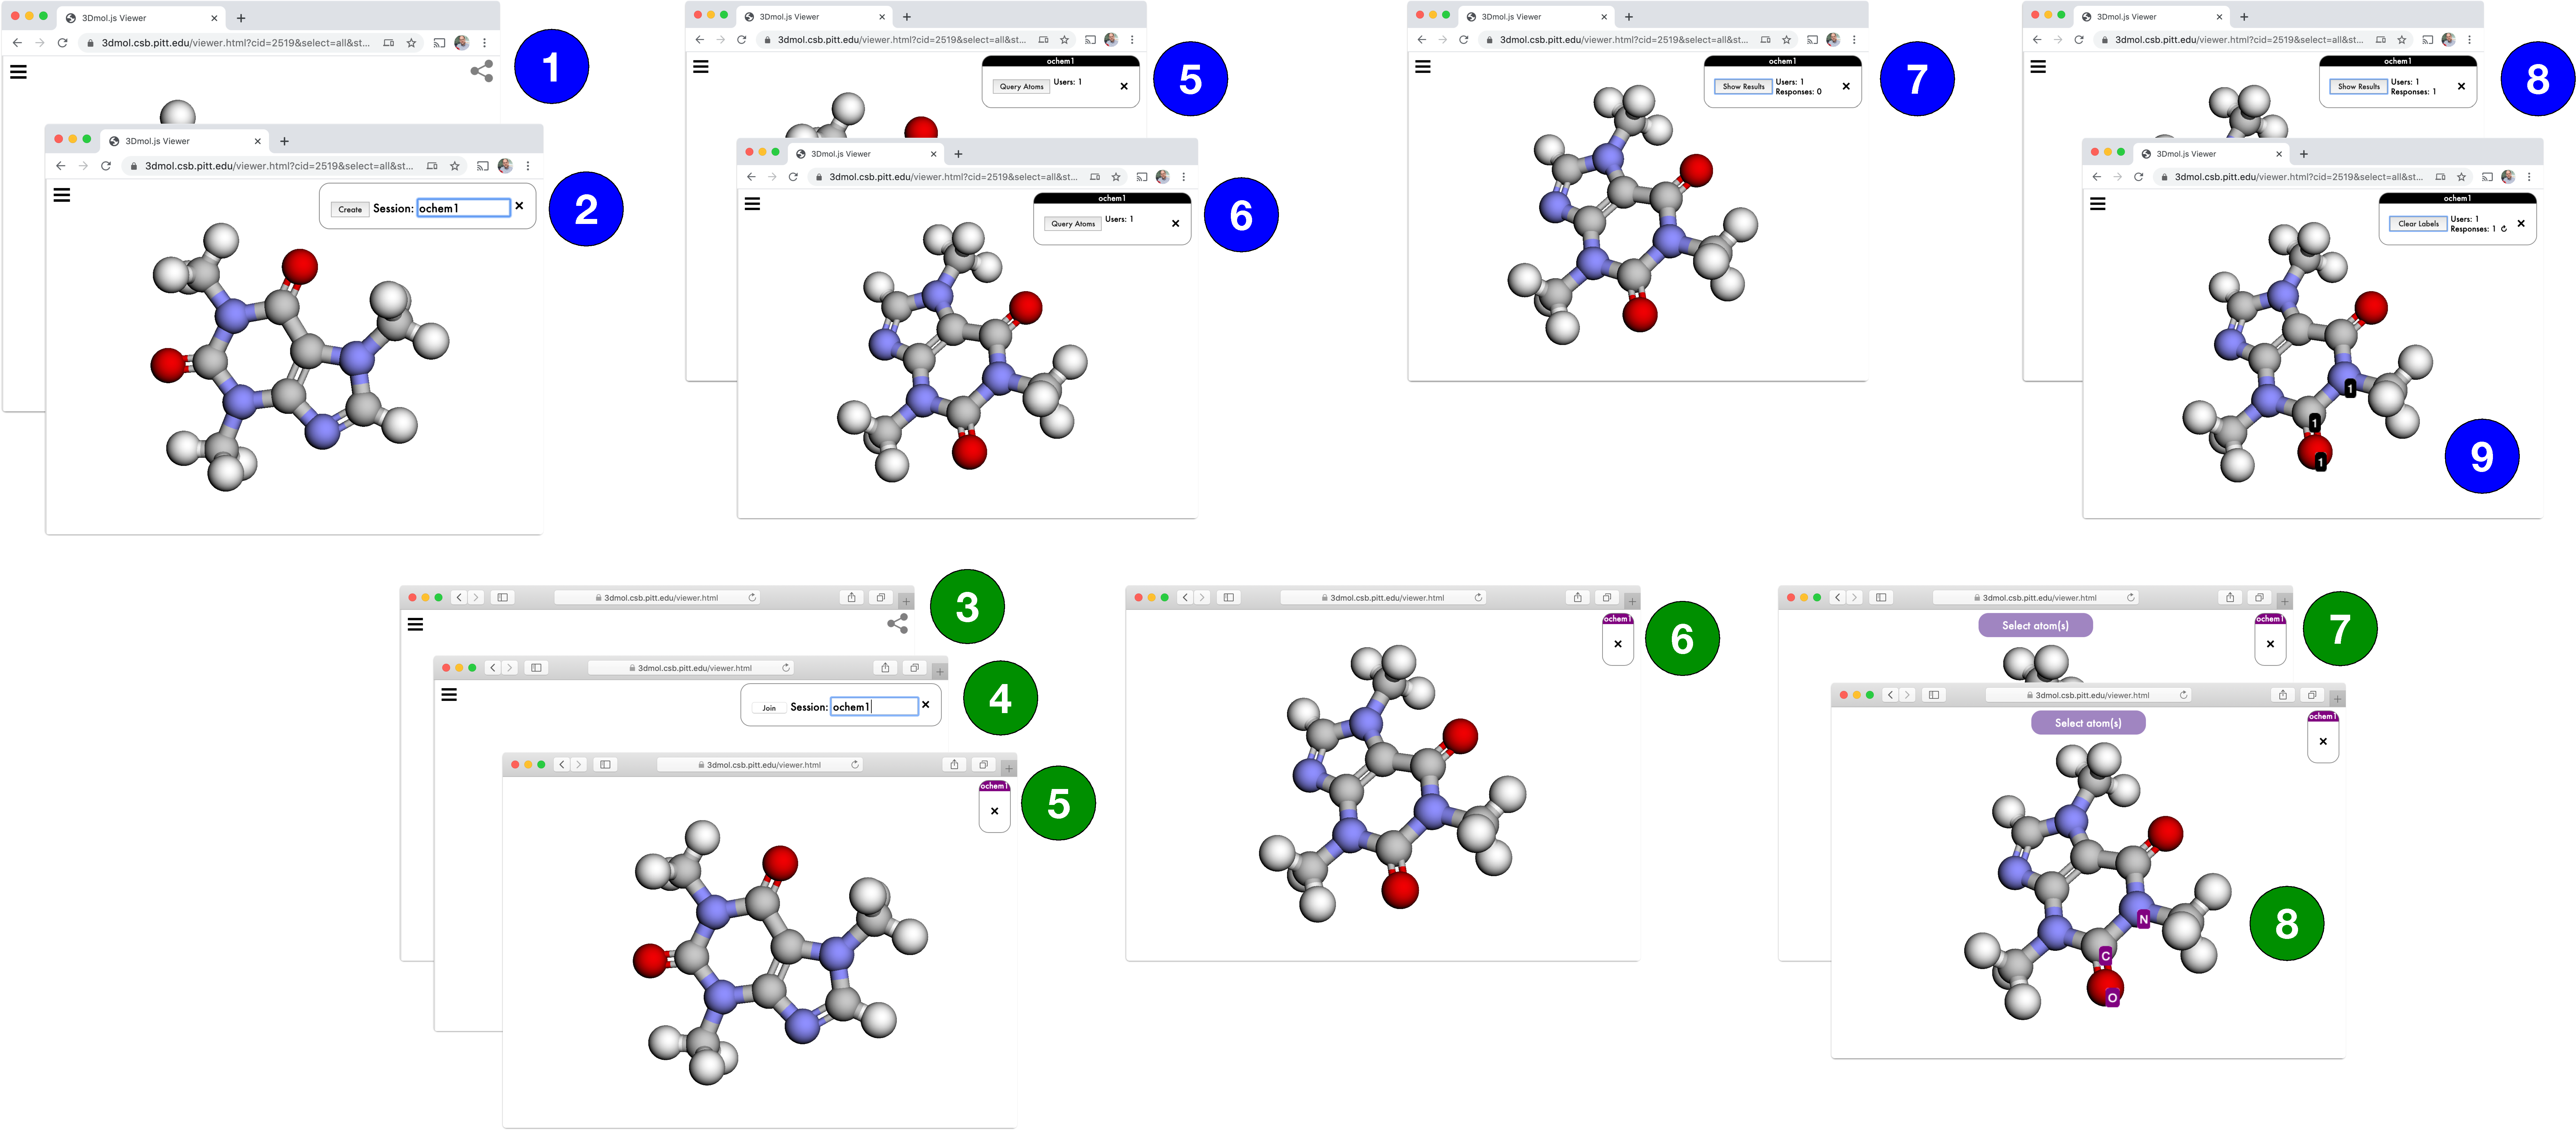
\includegraphics[width=\linewidth]{flow}
    \caption{Flow of instructor (top) and student (bottom) interactions with the 3Dmol.js classroom response system.}
    \label{fig:flow}
\end{figure}

\subsection{User Interface}

Usage of the 3Dmol.js learning environment is shown in Figure~\ref{fig:flow}.  (1) The instructor clicks on the `share' icon in the upper right of the hosted viewer. (2) In the resulting text box, the instructor creates a session by specifying its name.  Once created, a session lasts as long as the creating browser window is left open and only that browser window has the ability to manipulate the session contents.  The session will be initialized with the current molecular view. If a session is already available, the `Create' button will change to a `Join' button.  (3) When students click on the share button (4) they enter the name of the already created session and click `Join.'  Alternatively, students can be provided with a URL of the form \url{http://3dmol.csb.pitt.edu/viewer.html?session=NAME} where NAME is the name of the session.  Note that the session must be extant for for this to be a valid URL. (5) This populates their viewer with the instructor's molecular view and the instructor's view is updated to show that an additional user has connected.  Monitoring the number of connections is important for ensuring the whole class is participating.  (6) When the instructor modifies the view of the molecule, the student's view is updated to match.  As long as the instructor is not changing the view, students can freely interact with the molecule by rotating, translating, or zooming the view. (7) When the instructor clicks on `Query Atoms' every student is prompted to `Select atom(s).'  (8) As students click on atoms, the number of responses is reported to the instructor.  When students select atoms they are labelled.  Students can deselect an atom by clicking on it again.  The number of responses is the number of students who have made any selection, not the number of selected atoms. (9) Once satisfied with the number of responses, the instructor can click `Show Results' and atoms in the instructor view will be labeled with the number of students who have clicked on them.  The opacity of the label is scaled proportionally to the popularity of the selection.  There is a refresh button available to load the most recent results, for example after further explaining a concept in response to the previously shown selections.  Once the answers have been discussed, the results can be cleared to pose a new question, or a different molecule can be loaded using the edit panel.


\subsection{Implementation}

3Dmol.js relies on the availability of WebGL, a JavaScript interface to OpenGL that enables hardware accelerated 3D graphics in the browser.  All modern browsers support WebGL 1.0, although currently some browsers (e.g. Internet Explorer, some mobile browsers) do not fully support WebGL 2.0 which is required for volumetric rendering in 3Dmol.js.  3Dmol.js supports touch controls (drag to rotate, pinch to zoom, three finger drag to translate) and so can be used on mobile devices, although some older devices with limited graphics processing power may not support WebGL.

Sessions are implemented using WebSockets, which is a low overhead communication protocol for maintaining a full duplex connection between a web browser and a server.  It does not require polling, reducing the computational load on both the client and server. The server managing the sessions is written in Python using Flask and SocketIO.  As with the rest of 3Dmol.js, the server source code is open source and so can be deployed locally if so desired instead of using the public \url{http://3dmol.csb.pitt.edu} website. The server stores the state of the session (the molecular data, the applied styles, and the viewer orientation) as updates are sent from the instructor as well as responses to queries as updates are sent from the students.  Sessions end when the instructor disconnects, freeing the memory occupied by the session state.


\section{Future Plans}

The 3Dmol.js learning environment already provides the necessary features to be fully usable in a chemistry classroom.  However, there are number of ways the software could be improved.  Currently, the hosted viewer and URL API does not support a grid view where there are multiple independent viewers shown on the same page.  In order to have students answer questions that select between different molecules (e.g., ``Which molecule is a disaccharide?''), a multi-molecule file must be used. In this case, the molecules are part of the same coordinate system and so can not be independently manipulated.  We would like to change this so not only can multiple molecules be independently displayed, but questions can be posed where students select whole molecules, not single atoms.  Other ideas for improved selection semantics are to allow students to select whole residues, e.g. amino acids of protein, for biochemistry applications.  Currently, if a molecule is not available in a public database, the user most host the molecular data themselves.  Although this can easily be done by uploading to public folders in file sharing services, we are considering supporting file uploads natively within the viewer.  Uploaded files would be associated with a unique identifier and permanently stored on the server.  Another future goal is to integrate with Jupyter notebooks.  3Dmol.js viewers can already be embedded in a Jupyter notebook using the py3Dmol module, but we would like to support learning environment features within notebooks as well.  This would allow instructors who create slides using Jupyter to embed the active learning activities directly within the lecture materials. We already provide a small JavaScript plugin that provides this functionality for multiple choice questions (\url{https://github.com/dkoes/asker.js}).  
 We strongly encourage users of the 3Dmol.js learning environment to provide feedback and suggestions on the project's GitHub Issues page (\url{https://github.com/3dmol/3Dmol.js/issues}).
 


%%%%%%%%%%%%%%%%%%%%%%%%%%%%%%%%%%%%%%%%%%%%%%%%%%%%%%%%%%%%%%%%%%%%%
%% The "Acknowledgement" section can be given in all manuscript
%% classes.  This should be given within the "acknowledgement"
%% environment, which will make the correct section or running title.
%%%%%%%%%%%%%%%%%%%%%%%%%%%%%%%%%%%%%%%%%%%%%%%%%%%%%%%%%%%%%%%%%%%%%
\begin{acknowledgement}



We thank Keshavan Seshadri for his contributions to the project during the Google Summer of Code.
  This work is supported by R01GM108340 from the National Institute of General Medical Sciences.

\end{acknowledgement}

%%%%%%%%%%%%%%%%%%%%%%%%%%%%%%%%%%%%%%%%%%%%%%%%%%%%%%%%%%%%%%%%%%%%%
%% The same is true for Supporting Information, which should use the
%% suppinfo environment.
%%%%%%%%%%%%%%%%%%%%%%%%%%%%%%%%%%%%%%%%%%%%%%%%%%%%%%%%%%%%%%%%%%%%%
%\begin{suppinfo}
%\end{suppinfo}

%%%%%%%%%%%%%%%%%%%%%%%%%%%%%%%%%%%%%%%%%%%%%%%%%%%%%%%%%%%%%%%%%%%%%
%% The appropriate \bibliography command should be placed here.
%% Notice that the class file automatically sets \bibliographystyle
%% and also names the section correctly.
%%%%%%%%%%%%%%%%%%%%%%%%%%%%%%%%%%%%%%%%%%%%%%%%%%%%%%%%%%%%%%%%%%%%%
\bibliography{references}

\end{document}